%Review notes for the beginning of ST 512
\begin{center}\large\textbf{Readings: Chapters 1-8 as needed}\\
\normalsize \end{center}
\large \hlinewd{2pt}
~\\\noindent \textbf{Big ideas in stats:}\normalsize\\~\\
\begin{itemize}
\item \underbar{Population} - all the values, items, or individuals of interest\\~\\

\item \underbar{Parameter}  - a (usually) unknown summary value about the population\\~\\

\item \underbar{Sample} - a subset of the population we observe data on\\~\\

\item \underbar{Statistic} - a summary value calculated from the sample observations
\end{itemize}

\begin{center}
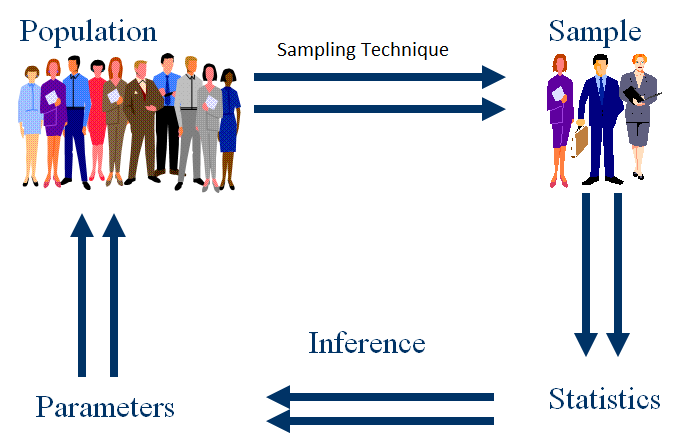
\includegraphics[scale=0.4]{paradigm}
\end{center}
Examples of paramters - (true) mean $\mu$, (true) variance $\sigma^2$.\\
Examples of statistics - sample mean $\bar{y}$, sample variance $s^2=\frac{\sum_{i=1}^{n}(y_i-\bar{y})^2}{n-1}$\\
Inference - Making mathematically sound claims about the poulation using sample data.

\newpage

\large \noindent \textbf{Scales (Types) of Data:}\normalsize\\~\\

\begin{itemize}
\item \underbar{Qualitative or Categorical} - A variable that is described by attributes or labels\\
\indent Subscales: \\
Nominal - categories have no ordering (Male, Female)\\
Ordinal - can order categories (Lickert scale data)\\~\\
\item \underbar{Quantitative} - A variable that is described by numerical measurements where arithmetic can be performed\\
\indent Subscales: \\
Discrete - finite or countable finite number of values (\# of flowers on a plant, 0, 1, 2, ...)\\
Continuous - any value in an interval is possibel (Temperature, $(-459.67\deg F, \infty)$
\end{itemize}

\large \noindent \textbf{Random Variables and Things of Interest:}\normalsize\\~\\
\begin{itemize}
\item \underbar{Random Variable (RV)} - Function that takes in outcomes from an experiment and outputs real numbers, or a numeric outcome to a random process\\~\\
\textbf{Things of interest}\\~\\
\begin{itemize}
\item \underbar{Distribution} - pattern and frequency of observable values\\
For continuous RVs, visualized with a smooth curve.
\item \underbar{Mean/Median} - measures of center of the distribution\\~\\
Focus on mean: true mean $\mu$, RV sample mean $\bar{Y}$, observed sample mean $\bar{y}$
\item \underbar{Standard Deviation, Variance, IQR, Range} - measures of spread for the distribution\\~\\~\\
Focus on SD and Variance: true variance $\sigma^2$, true SD $\sigma$, observed sample variance $s^2$, observed SD $s$
\end{itemize}
\end{itemize}

\large \textbf{Graphical Descriptions of RV`s:}\normalsize\\~\\
\begin{itemize}
\item \underbar{Histogram} - Graphs the frequencies or relative frequencies of realizations of a RV\\~\\
\item \underbar{Boxplot} - Uses the Five Number Summary to display the realizations of a RV\\
Five number summary: $min,~Q_1,~M,~Q_3,~max$
\end{itemize}

\begin{center}
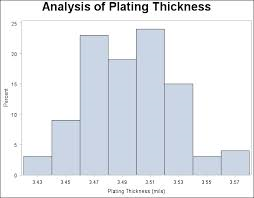
\includegraphics[width=2.8in, height=2.2in]{histogram}~~~~~~~~~~~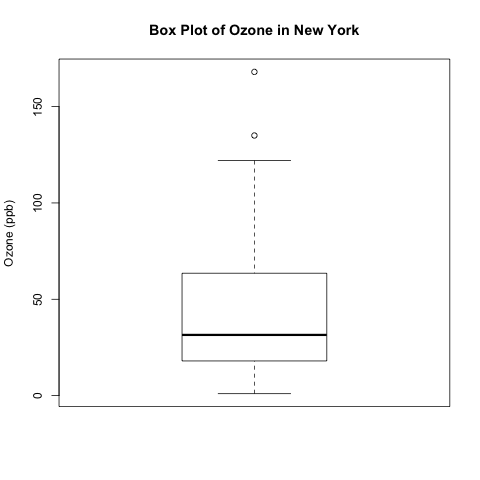
\includegraphics[width=2.8in, height=2.4in]{boxplot}
\end{center}

~\\~\\
\large \textbf{Statistics are also RVs.  The distribution of a statistic is called a} \underbar{sampling distribution}\normalsize\\
\textbf{Central Limit Theorem (CLT):}\\~\\
If a RV $Y$ has a (true) mean $\mu$ and (true) variance $\sigma^2$, and a random sample is of size $n\geq 30$ is taken then
$$\bar{Y}\sim N(\mu,\sigma^2/n)$$
Note: If $Y\sim N(\mu,\sigma^2)$ then $\bar{Y}\sim N(\mu,\sigma^2/n)$ for any $n$.\\~\\

\noindent\large \textbf{2 main ways to make inference about a (true) mean,} $\mu$:\normalsize\\
\begin{enumerate}
\item When the true SD, $\sigma$, is known we looked at the sampling distribution of the statistic\\~\\
$Z=\frac{\bar{Y}-\mu}{\sigma/n} \sim N(0,1)$~~~valid if $\bar{Y}$ has a normal distribution\\~\\
Allows us to form a CI:	\hspace{2in}		And a test statistic: Testing $H_0: \mu=\mu_0$\\~\\
$\bar{y}\pm z_{\alpha/2}\sigma/\sqrt{n}$ \hspace{2.5in} $z_{obs}=\frac{\bar{y}-\mu_0}{\sigma/\sqrt{n}}$\\

\item When the true SD, $\sigma$, is unknown we looked at the sampling distribution of the statistic\\~\\
$T=\frac{\bar{Y}-\mu}{s/n} \sim t_{n-1}$~~~valid if $\bar{Y}$ has a normal distribution, allow for $n\geq 15$ or so in CLT\\~\\
Allows us to form a CI:	\hspace{2in}		And a test statistic: Testing $H_0: \mu=\mu_0$\\~\\
$\bar{y}\pm t_{(n-1,\alpha/2)}s/\sqrt{n}$ \hspace{2.4in} $t_{obs}=\frac{\bar{y}-\mu_0}{S/\sqrt{n}}$\\
\end{enumerate}

\newpage

\noindent\large \textbf{Inference about two (true) means, $\mu_1$ and $\mu_2$:}\normalsize\\
\begin{itemize}
\item	From paired samples, $x_1, x_2,..., x_n$ and $y_1, y_2,..., y_n$ where difference is normally distributed\\~\\
CI: $(\bar{x}-\bar{y})\pm t_{(n-1,\alpha/2)}s_{diff}/\sqrt{n}$\\~\\
HT: $H_0: \mu_1=\mu_2,$ i.e. $\mu_1-\mu_2=0$~~~~$t_{obs}=\frac{(\bar{x}-\bar{y})-0}{s_{diff}/\sqrt{n}}$
\item Two separate samples from normal populations, $x_1, x_2,..., x_n$ and $y_1, y_2,..., y_n$\\~\\
CI: $(\bar{x}-\bar{y})\pm t_{(\nu,\alpha/2)}\sqrt{s_{_X}^2/n+s_{_Y}^2/m}$ where $\nu$ is an estimate of df\\~\\
HT: $H_0: \mu_1=\mu_2,$ i.e. $\mu_1-\mu_2=0$~~~~$t_{obs}=\frac{(\bar{x}-\bar{y})-0}{\sqrt{s_{_X}^2/n+s_{_Y}^2/m}}$
\end{itemize}

~\\

\noindent\large \textbf{Extension to inference about t (true) means, $\mu_1, \mu_2, ..., \mu_t$:}\normalsize\\
Balanced One-way ANOVA table (same number of replicates per group)\\
\begin{center}
\begin{tabular}{c|c|c|c|c|c}
Source & DF & SS & MS & F-stat & P-value\\
\hline& & & & &\\
Treatment & $t-1$ & $n\sum_{i=1}^{t}(\bar{Y}_{i+}-\bar{Y}_{++})^2$ & $\frac{SS(Trt)}{t-1}$ & $\frac{MS(Trt)}{MS(E)}$ & Use $F(t-1,t(n-1))$\\& & & & &\\
Error & $t(n-1)$ & $\sum_{i=1}^{t}\sum_{j=1}^{n}(Y_{ij}-\bar{Y}_{i+})^2$ & $\frac{SS(E)}{t(n-1)}$ &  & \\& & & & &\\
Total & $nt-1$ & $\sum_{i=1}^{t}\sum_{j=1}^{n}(Y_{ij}-\bar{Y}_{++})^2$ & & & \\
\end{tabular}
\end{center}

~\\~\\Analysis used for a completely randomized design.  \\~\\
P-value tests $H_0: \mu_1=\mu_2=...=\mu_t$ vs $H_A:$ at least 1 mean differs\\~\\
One Way ANOVA model:\\
$$Y_{ij}=\mu+\alpha_i+E_{ij}$$
where $i=1,2,...t$ and $j=1,2,...,n$ (total sample size = $nt=N$)\\~\\
$\mu$ = overall mean\\
$\alpha_i$ = effect from group i\\
 $E_{ij}$ = random error assumed to be $iid~N(0,\sigma^2)$

\newpage

\large \textbf{For two quantitative variables measured on the same units, the linear relationship can be investigated:}\normalsize\\~\\
Simple linear regression model $Y_i=\beta_0+\beta_1x_i+E_i$ or use correlation.\\~\\~\\

\large \textbf{For a hypothesis test, the p-value means}\normalsize\\~\\
probability of observign a test statistic as extreme or more extreme than the one observed, assuming the null hypothesis is true.\\~\\~\\

\large \textbf{For a given a null hypothesis, statistical significance implies}\normalsize\\~\\
the observed value was unlikely to have occurred by random chance alone (assuming the null hypothesis is true).\\~\\~\\

\large \textbf{For an observed confidence interval (cL, cU) we can say}\normalsize\\~\\
We are \underbar{~~~~~}\% confident the true parameter value is contained in the interval.  (***Do not say probability or chance!)\\~\\~\\

\large \textbf{The idea of Confidence means}\normalsize\\~\\
The procedure used to create the interval has a \underbar{~~~~}\% probability of producing an interval that contains the parameter.\\~\\
i.e. If the experiment were done repeatedly and an interval made for each sample, \underbar{~~~~}\% of the intervals would contain the parameter value.

